\subsection{The Projected Grid Concept}
The projected grid is based on a simple concept: in order to achieve an
uniform distribution of details on the image plane, an uniformly spaced grid is
created in post-perspective space and transformed back to world space.
Figure~\ref{fig:projectedgrid} illustrates the difference between a classic
world space approach and the projected grid.
\begin{figure}
\centering
\subbottom[Increase]
{
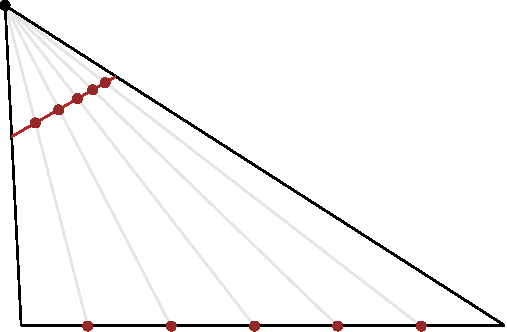
\includegraphics[scale=0.75]{figures/ProjectedGridVsWorldSpace.pdf}
\label{fig:subfigprojgrid1}
}
\subbottom[Increase]
{
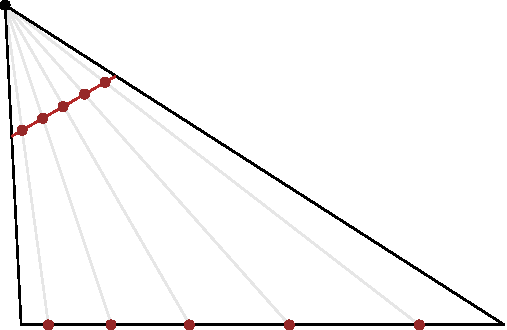
\includegraphics[scale=0.75]{figures/ProjectedGridUniform.pdf}
\label{fig:subfigprojgrid2}
}
\caption[The Projected Grid Concept]{The image on the left
~\subcaptionref{fig:subfigprojgrid1} shows an uniform grid in worldspace, it's
projection onto the image plane is not uniformly spaced though. The image on the
right~\subcaptionref{fig:subfigprojgrid2} on the other hand depicts an uniform grid on
the image plane and it's associated non-uniform spaced worldspace positions.}
\label{fig:projectedgrid}
\end{figure}
